\documentclass[12pt, a4paper]{article}
\usepackage[utf8]{inputenc}
\usepackage[russian]{babel}
\usepackage[T2A]{fontenc}
\usepackage{amsfonts}
\usepackage{amsmath}
\usepackage{indentfirst}
\usepackage{amsthm}
\usepackage{float} 
\DeclareMathOperator*{\argmin}{argmin}
\newtheorem{lemma}{Утверждение}[section]

\usepackage[left=2cm,right=1.5cm,top=2cm,bottom=2cm]{geometry}
\linespread{1.25}

\usepackage{graphicx}
\graphicspath{{pictures/}}
\DeclareGraphicsExtensions{.pdf,.png,.jpg}

\begin{document}
\pagestyle{empty}

\begin{center}
	ФЕДЕРАЛЬНОЕ ГОСУДАРСТВЕННОЕ БЮДЖЕТНОЕ ОБРАЗОВАТЕЛЬНОЕ\\
	УЧРЕЖДЕНИЕ ВЫСШЕГО ОБРАЗОВАНИЯ\\
	<<МОСКОВСКИЙ ГОСУДАРСТВЕННЫЙ УНИВЕРСИТЕТ\\
	имени М.\,В.~ЛОМОНОСОВА>>
\end{center}
\vspace{4pt}
\begin{center}
	МЕХАНИКО-МАТЕМАТИЧЕСКИЙ ФАКУЛЬТЕТ
\end{center}
\vspace{4pt}
\begin{center}
	КАФЕДРА ВЫЧИСЛИТЕЛЬНОЙ МАТЕМАТИКИ
\end{center}
\vspace{1cm}
\begin{center}
	ВЫПУСКНАЯ КВАЛИФИКАЦИОННАЯ РАБОТА\\
	специалиста
\end{center}

\begin{center}
	\textbf{ПОСТРОЕНИЕ ОПТИМАЛЬНОГО МАРШРУТА \\
		ПРИ ЗАДАННОЙ МОДЕЛИ ДВИЖЕНИЯ ДРУГИХ \\
		УЧАСТНИКОВ ТРАНСПОРТНОЙ СЕТИ}
\end{center}
\vspace{1cm}
\begin{center}
	\begin{tabular}{p{9cm} l}
		& Выполнил студент $610$ группы\\
		& Разумова Любовь Евгеньевна\\
		& $\phantom{C_n^k=C_n^{n-k}}$\\
		& $\underline{\phantom{\int\limits_a^bf(x)dx=F(b)-F(a)}}$\\
		& подпись студента\\
		& $\phantom{\int\limits_f(z)dz=0}$\\
		& Научный руководитель:\\
		& доктор физико-математических наук \\
		& Афонин Сергей Александрович\\
		& $\phantom{C_n^k=C_n^{n-k}}$\\
		& $\underline{\phantom{\int\limits_a^bf(x)dx=F(b)-F(a)}}$\\
		& подпись научного руководителя\\
	\end{tabular}
\end{center}
\vspace{1cm}
\begin{center}
	Москва\\
	$2022$
\end{center}

\newpage
\pagestyle{plain}
\tableofcontents{}

\newpage	

\section*{Введение}

В данной работе рассматривается задача нахождения наилучшего в каком-то смысле пути с учетом движения фиксированного количества участников по заданным ранее маршрутам в условиях ограниченности модели дорожной системы. Новый построенный маршрут должен отвечать выбранным критериям кратчайшести среди всевозможных путей на всем временном промежутке, но не обязательно в каждый момент времени. Знание маршрутов изначальных участников помогает определить плотность автомобильного потока на конкретных отрезках пути. Рассматриваемая модель приближена к реальной дорожной системе городов, поэтому на всех ее участках наложены ограничения по вместимости участников и скорости их движения. Такие ограничения влияют на показатели маршрутов участников, такие как итоговое время движения и длину пути. 


Тема актуальна в наше время, так как она помогает решить проблему пробок на дорогах, а также призвана упростить водителям выбор маршрута, который займет у них наименьшее время. Задача имеет практический характер... Проблема пробок в Москве стоит очень остро, ученые решают ее не первый год..

В мире прогнозы загруженности используются для автоматического управления дорожным движением в некоторых городах. Первые прототипы, в которых были применены прогнозы, появились появились в 1998 году в США. А первое пилотное использование системы, «заглядывающей в будущее», началось в 2006 году в Сингапуре. Среди наших соотечественников похожей задачей занимается отдел навигации Яндекса. Разработчики собирают информацию по трекам движения автомобилей, осуществляют привязку треков к ребрам графа дорожной сети, вычисляют некоторую усредненную скорость на отдельных участках, рисуют карту прогноза дорожной ситуации на ближайший час и в связи с этим предлагают оптимальный по времени путь, а также еще пару алтернативных маршрутов. Сложность сбора информации и построения треков движения состоит в том, что, во-первых, не все пользуются сервисами Яндекса при построении своего маршрута, и во-вторых, в данных постоянно возникают лишние шумы, что приводит к выбросам на графиках, и с таким качеством информации работать очень сложно. Мы же рассматриваем более прозрачную и простую модель, когда все маршруты изначально проложены и нам известны, и они не меняются с течением времени. Это не умаляет значимости и важности поставленной нами задачи. Мы получим более четкие результаты, идеи в дальнейшем могут развиваться и открывать новые возможности для более широкой задачи, например, как у Яндекса. Также стоит отметить, что специалисты по навигации используют статистические методы и машинное обучение в качестве инструмента для решения своих задач, мы же подойдем к вопросу с другой стороны и применим другие алгоритмы. На данный момент отдел навигации Яндекса проводит улчшения своих методов и подходов к решению задач, а также придумывает какие-то новые метрики и способы оценки качества этих решений.


Задачи, которые мы ставили перед собой в рамках выбранной темы дипломной работы: формальная постановка задачи, анализ полученных ранее результатов в этой теме, разработка простого алгоритма решения на основе моделирования и его оценка, оценка устойчивости полученного решения, попытка обощения дорожной сети, ее расширение (или сужение?). Методы исследования включают в себя: построение графа с вершинами в концевых точках заданных маршрутов и ребрами, отображающими дороги между ними, определение функции веса-загруженности дорог, 



Основа нашей задачи - нахождение наилучшего пути в условиях изменчивости плотности и скорости дорожного потока на участках в заисимости от времени.

В первой главе вы сможете ознакомиться с деталями поставленной задачи, далее мы решим ее путем моделирования дорожной ситуации и применением некоторых известных алгоритмов, в третьей главе поговорим о достоинствах и недостатках такого решения, его сложности и реализуемости в реальной жизни. Четвертая глава будет содержать описание некоторых модификаций графа дорожной сети, а также улучшений решения на таком графе. В завершении поделимся результатами проделанной работы, оценим их качество и сделаем выводы.




\newpage
\section{Постановка задачи}
Пусть задан ориентированный \textit{граф дорожной сети} $ G (V, E, l)$ таким образом, что вершины $ v \in V$ осуществляют роль перекрестков, а ребра $e \in E$ - роль дорог. Каждое ребро имеет длину, т.е. задана функция $l : E \rightarrow \mathbb {R} $. Также задана \textit{модель движения} АТС -- набор правил, определяющих поведение участников в зависимости от ситуации на дороге.

Пусть имеется $n$ участников, которые движутся по заранее заданным маршрутам:  $ p_i = \langle E^i_{j_1}, E^i_{j_2}, \dots, E^i_{j_{m_i}} \rangle$, $ E^i_{j_k} \in E \quad i = 1, \dots, n$. Добавим к ним $(n+1)$-ого участника, которому нужно добраться из пункта $A$ в пункт $B$, $A, B \in V$. Определим $P(A,B)$~-- множество всех простых путей из $A$ в $B$. Модель движения позволяет определить \textit{часть пройденного пути} для каждой АТС в зависимости от движения других участников, т.е. определить непрерывные монотонные функции
\begin{center}
 $x_i(G, p_1, \dots, p_n, p, \cdot ) : \mathbb {R} \rightarrow [0 , 1] $, $i = 1, \dots, n+1$, $p \in P(A, B) $.
\end{center}
Ввиду однозначной определенности последовательности ребер $p_j$ и графа дорожной сети $G$, явную зависимость $x_i$ от данных параметров можно не указывать.

На множестве путей $P(A,B)$ определим $T(p) = \displaystyle \inf_t \{t : x_{n+1}(p, t) = 1\}$~-- время прибытия $(n+1)$-ого участника в вершину $B$ при движении по маршруту $p$. Требуется найти такой путь $p^* \in P(A, B)$, что $T(p^*)$ - минимальна. Другими словами, для заданной модели движения на графе дорожной сети $G(V, E, l)$ при движении $n$ участников по путям $p_1, \dots, p_n$ требуется найти такой путь $p^*$ из $A$ в $B$, что движение нового участника по этому пути $p^*$ будет \textit{оптимально}, то есть
$$p^* = \argmin_{p \in P(A, B)} T(p).$$

\newpage
\section{Модели движения}

Формализуем понятие модели движения, упомянутое в постановке задачи. Обратимся к теории автоматов и с ее помощью попробуем описать правила движения АТС. Аналогичный подход использовали К.\,Нагель и М.\,Шрекенберг \cite{automat_baza}. В своей работе авторы рассматривают модель клеточных автоматов, которая предполагает разбиение дорог на клетки и использование дискретного времени. Эта идея нашла применение в описании движения физических частиц \cite{automat_phyz}, а также в исследовании пробок на дорогах \cite{automat_jam}. Мы же не будем ограничиваться клеточными автоматами и опишем случай непрерывного движения.

\textit{Моделью движения} АТС назовем $M = \left(n, G, S, F, \{t_i\}_{i = 1}^n, \{\varphi_i\}_{i = 1}^n \right)$, где $n$ - количество участников движения, $G$ --- граф дорожной сети, $S$ --- множество состояний, которые могут принимать участники, $F \subset S$ --- множество заключительных состояний, $t_i: S^n \rightarrow R_{>=0}$ --- функция критического момента движения участника $i$, $\varphi_i: S^n \times \mathbb{R}_{>= 0} \rightarrow S$ --- функция перехода состояния $i$-ого участника в некоторый момент времени $t$. Считаем, что попав в заключительное состояние, мы не можем его покинуть:
$$\varphi_i (s_1, \dots, s_i, \dots, s_n, t) = s_i, \text{ } s_1, \dots, s_n \in S, \text{ } s_i \in F, \text{ } \forall t \in \mathbb{R}_{\ge 0}.$$

Множество $S$ описывает текущий характер двжиения машины. Это, в первую очередь, ребро, на котором едет участник, координата на этом ребре и скорость участника. Если модель описывает некоторое измение ускорения, то под состоянием $s$ также имеется ввиду текущее ускорение машины. Подразумевается, что состояния можно разбить на классы, например <<свободное движение>>, <<ожидание>>, <<прибытие>>, <<торможение перед лидером>> и тд. Функция $t_i$ описывает время, когда участнику необходимо совершить переход из текущего состояния в состояние другого класса. 

Модель движения АТС можно описать некоторой диаграммой, описывающей переходы между классами для каждого участника. Диаграмма представляет собой ориентированный граф, где вершины --- классы состояний, а ребра являются переходами в другое состояние. Метка на ребре --- условие перехода, который осуществляется, если $t =  t_i(s_1, \dots, s_n)$ для некоторого $s_i$ из класса состояний. Непомеченные ребра соответствуют условию $t < t_i(s_1, \dots, s_n)$. Например, правила движения, в которых поведение участника зависит от расстояния, до впереди идущего участника может быть задано следующей диаграммой (см. рис. \ref{ris:example_diag}):

\begin{figure}[H]
	\centering
	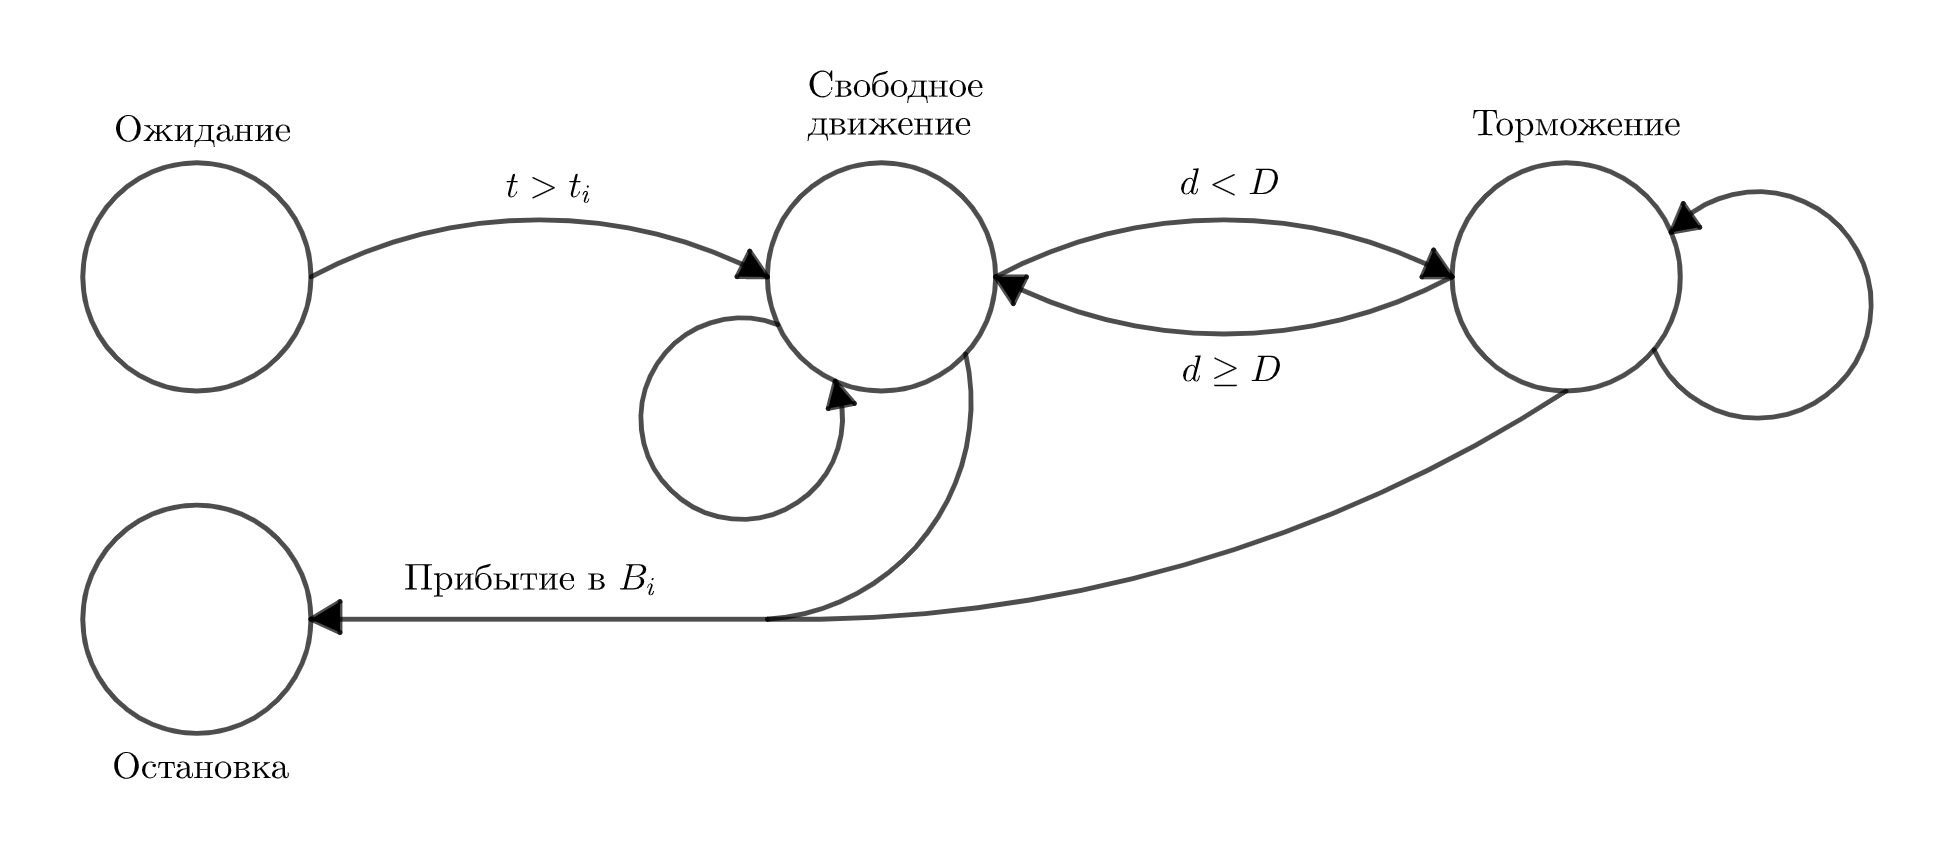
\includegraphics[scale=0.25]{Mur.png}
	\caption{Диаграмма для $i$-ого участника в модели движения, где $d$~-- расстояние до впереди идущего участника, $D$~-- максимальное расстояние взаимодействия с впереди идущим участником}
	\label{ris:example_diag}
\end{figure}

\if 0
%Нас интересует точное решение, поэтому промоделируем движение $n$ участников, чтобы в каждый момент времени были известны функции $x_i(t)$. 
Поведение движения АТС в нашей постановке задачи определяется некоторой системой правил. Представим примеры таких приавил, которые описывают естественный, близкий к реальности характер движения автомобилей.

Говоря о поведении движения автомобилей, мы имеем в виду изменение их скоростей в зависимости от ситуации на дороге. Для каждого АТС введем функцию \textit{скорости} \\ ${v_i(t) : \mathbb {R}_+ \rightarrow \mathbb {R}_+}$.  Обозначим через $v_m \in \mathbb {R}$ максимально возможную скорость, или \textit{скорость свободного движения}: $v_i(t) \leq v_m, \forall t \in \mathbb {R}, i = 1, \dots, n+1$.
\fi

Рассмотрим модели движения, в которых изменения скорости участников базируются только на количестве участников на ребре в момент времени $t$. Назовем такие модели \textit{макроскопическими}, а все остальные --- \textit{микроскопическими}. 

\subsection{Макроскопические модели}

При движении $n$ участников такие модели можно параметризовать набором действительных чисел $v_1, \dots, v_n$, где $v_k$~-- скорость при $k$ участниках на ребре. Множество состояний в макроскопических моделях движения можно разбить на $n$ классов по количеству участников на ребре. 

\subsection{Микроскопические модели}
Опишем модель \textit{следования за лидером}~-- модель, в которой поведение движения участника зависит от расстояния до впереди идущего АТС. 
Введем понятие \textit{дистанции видимости} $D$~---расстояние, на котором текущий участник начинает взаимодействовать с впереди идущим лидером. Также будем считать , что участники должны соблюдать \textit{безопасное расстояние} $l$~--- оказавшись на расстоянии $d \leq l$ до лидера, участник мгновенно сбрасывает свою скорость до нуля. Скорости участников будут изменяться посредством ускорений, положим
$$a_+ = \frac{v^2_m}{D}$$~--- ускорение такое, что позволяет разогнаться с нулевой до максимальной скорости за время, которое нужно для преодоления расстояния $D$ с постоянной максимальной скоростью. 
Также пусть $$a_- = -\frac{v^2_m}{2l}$$~--- торможение такое, что позволяет снизить скорость с максимальной до нуля, проехав расстояние $l$.

Пусть $i$~-ый и $(i+1)$~-ый участники, лидер и следующий за ним соотвественно, оказались в момент времени $t$ на расстоянии $d$ относительно друг друга со скоростями $v_i$ и $v_{i+1}$. Опишем характер их движения.
\begin{enumerate}
	\item $d \ge D $
	\begin{enumerate}
		\item $v_{i+1} = v_{max} \Rightarrow a_{i+1} = 0$, продолжаем ехать с максимальной скоростью.
		\item $v_{i+1} < v_{max} \Rightarrow a_{i+1} = a_+$ на время $t = \frac{v_{max}-v_{i+1}}{a_+}$, после чего $v_{i+1} = v_{max}, a_{i+1} = 0$
	\end{enumerate}	
	\item $d \leq l \Rightarrow v_{i+1} = 0$
	\item $l < d < D $
	\begin{enumerate}
	\item $v_{i+1} \leq v_i$
		\begin{enumerate}
			\item $a_i = 0$, т.е. его движение равномерно, это может быть только в 2-х случаях:
			\begin{enumerate}
				\item $v_i = v_{max} \Rightarrow a_{i+1} = a_+$ на время $t = \frac{v_{max}-v_{i+1}}{a_+}$, после чего $v_{i+1} = v_{max}, a_{i+1} = 0$
				\item $v_i = 0$, едем время $t = \frac{d-l}{v_{i+1}}$, не меняя скорость, после чего останавливаемся, $v_{i+1} = 0$.
			\end{enumerate}	
			\item $a_i \neq 0 \Rightarrow a_{i+1} = a_i$ 
		\end{enumerate}
	\item $v_{i+1} > v_i$ 
	\begin{enumerate}
		\item $a_i = a_+ \Rightarrow a_{i+1} = a_-$ до момента, когда $v_i + a_it = v_{i+1} + a_{i+1}t$ или $v_{i+1}$ станет $0$, т.е. до $t = min\left(\frac{2Dl(v_{i+1}-vi)}{v^2_{max}(l+D)}, \frac{2lv_{i+1}}{v^2_{max}}\right)$,  после чего $a_{i+1} = a_i = a_+$. 
		\item $a_i = a_- \Rightarrow a_{i+1} = a_i = a_-$.
	\end{enumerate}	
	\end{enumerate}
\end{enumerate}

\newpage
\section{Моделирование}

Под моделированием будем понимать воспроизведение движения всех АТС по установленным правилам. Рассмотрим 2 различных способа моделирования с $(n+1)$-ым участником: 
\begin{enumerate}
	\item он влияет на движение $n$ участников и вследствие на самого себя;
	\item движение $n$ участников не зависит от добавленного АТС.
\end{enumerate}

\subsection{Независимость движения участников от добавленного АТС}
\subsection{Взаимосвязь движений нового участника и группы АТС}

\newpage
\section{Поиск оптимального пути}

Отметим, что количество путей конечно, поэтому первое, что приходит на ум в качестве решения, это перебор всех возможных путей и нахождение подходящего по затраченному времени. Посчитаем сложность этого алгоритма и сделаем вывод о его использовании в нашей задаче на практике.

\subsection{Перебор. Сложность}
Чтобы узнать, применим ли перебор в нашем случае, посчитаем сложность нахождения кратчайшего пути среди множества всех простых путей из $A$ в $B$. Пусть $S_x(p)$~-- сложность моделирования, т.е. нахождения функции $x^p_{n+1}(t)$, при выборе пути $p$. Тогда сложность перебора
\begin{center}
 $S = \sum\limits_{p \in P(A,B)} S_x(p) = \vert P(A,B) \vert * \overline S_x$, где $\overline S_x$~-- средняя сложность.
\end{center}
Заметим, что $ S $ растет при увеличении количества возможных путей. Так, в полном графе на $\vert V \vert$ вершинах получим $S = 2^{|V|-2} * \overline S_x$.

В качестве примера можем рассмотерть также регулярный граф-решетку на $\mathbb {R}^2$ и на нем оценить снизу сложность поиска пути с минимальными тратами. Пусть точки $A$ и $B$ имеют координаты $(a_1, a_2)$ и $(b_1, b_2)$ соответственно. Тогда количество путей минимальной длины в метрике Манхэтенна будет составлять $C^{|a_1-b_1|}_{|a_1-b_1| + |a_2-b_2|}$. Понятно, что путей $|P(A,B)|$ в таком графе гораздо больше. Таким образом, получаем оценку снизу для регулярного решеточного графа

\begin{center}
	$C^{|a_1-b_1|}_{|a_1-b_1| + |a_2-b_2|} * \overline S_x  \leq  \vert P(A,B) \vert * \overline S_x = S$.
\end{center}

Например, в решетке-квадрате со стороной $m$ при движении из угловой точки по диагонали в угловую точку напротив количество путей минимальной длины составит $C^m_{2m} = \frac{(2m)!}{m!m!} $. По формуле Стирлинга
\begin{center}
 $ C^m_{2m} = \frac{\sqrt{2\pi(2m)} \left( \frac{2m}{\exp} \right)^{2m}}{\left(\sqrt{2\pi m} \left( \frac{m}{\exp} \right)^m \right)  \left(\sqrt{2\pi m} \left( \frac{m}{\exp} \right)^m \right)} = \frac{2\sqrt{\pi m} \left( \frac{2m}{\exp} \right)^{2m}}{2\pi m \left( \frac{m}{\exp} \right)^{2m}} = \frac{2^{2m}}{\sqrt{\pi m}}$.
\end{center}
Понятно, что при увеличении $m$, количество путей экспоненциально растет.

С помощью перебора можно находить кратчайшие пути быстро, если $|P(A,B)|$ не велико. Однако изначально наша задача была сформулирована в терминах дорожной сети и предполагала графы с достаточно большим количеством вершин и ребер, что влияет на количество маршрутов для заданных точек. Таким образом, можно сделать вывод, что в общем случае перебор путей в нашей задаче на практике не применим.

\newpage
\subsection{Дейкстра}


Рассмотрим вспомогательную задачу. Пусть на каждом ребре $e \in E$ графа $G(V, E)$ определена функция \textit{временных затрат} $\phi_e(t) : \mathbb {R}_+ \rightarrow \mathbb {R}_+$. Если мы оказались в начальной вершине ребра $e$ в момент времени $t$, то время преодоления ребра будет равняться $\phi_e(t)$. Рассмотрим путь $p = \langle V_0, e_1, V_1, e_2, V_2, \dots, V_{k-1}, e_k, V_k \rangle $ и начало движения происходит в вершине $V_0$ в момент времени $t_0 = t$, тогда
\begin{align*}
t_0 & = t  \\
t_1 & = \phi_{e_1}(t) + t = \phi_{e_1}(t_0) + t_0  \\
t_2 & = \phi_{e_2}(\phi_{e_1}(t) + t) + \phi_{e_1}(t) + t = \phi_{e_2}(t_1) + t_1 \\
    & \dots \\
t_i & = \phi_{e_i}(t_{i-1}) + t_{i-1} \\
    & \dots \\
t_k & = \phi_{e_k}(t_{k-1}) + t_{k-1}
\end{align*}
Пусть $P(A, B)$~-- множество всех простых путей из $A$ в $B$ в графе $G(V, E)$. Необходимо найти путь из $A$ в $B$, который требует минимальных затрат, т.е. 
$$T = \min_{p \in P(A, B)} t_{|p|}.$$
В общем случае функции временных затрат могут быть любыми. Давайте рассмотрим эту задачу с дополнительным условием на $\phi_e(t):$
$$ \phi_e(t) \leq \Delta + \phi_e(t + \Delta), \quad \Delta \ge 0$$
Назовем это условие \textit{неравенством прохождения ребер}. Утверждается, что если для $\forall e \in E$ функции временных затрат $\phi_e$ удовлетворяют неравенству прохождения ребер, то задачу можно решить модифицированным алгоритмом Дейкстры.

\subsubsection{Модифицированный алгоритм Дейкстры}

$\textbf{Алгоритм построения минимального маршрута}$

Для каждой вершины будем хранить два значения: минимальное время, за которое можно добраться до этой вершины, и ребро, через которое проходит кратчайший маршрут до вершины.
Применяем стандартный алгоритм Дейкстры, с отличием, что при посещении вершины мы фиксируем время для нее и пересчитываем функции временных затрат на всех ребрах, исходящих из этой вершины.\\
Для запуска алгоритма потребуется задать начальное время - минимальное время в точке старта. Это можно использовать в анализе маршрута.


\begin{lemma}
Данный маршрут обладает наименьшим временем прохождения.
\end{lemma}

\begin{proof}

Будем доказывать по индукции :\\
База индукции - в графе 2 вершины и несколько ребер между ними. Минимальным маршрутом будет то ребро, у которого наименьшее время прохождения.\\
Шаг индукции - считаем что в случае с m (< n) вершинами лемма справедлива. Рассмотрим граф, содержащий n вершин. Пусть $\exists$ маршрут P в этом графе, требующий меньше затрат, чем построенный нашим алгоритмом, тогда возьмем ближайшую к началу точку, обозначим ее $C$, в которой выбрано ребро, отличное от минимального по затратам. Очевидно, что если точка $C$ совпадает с точкой $F$, концом маршрута, то P не является минимальным по времени прохождения. \\
Пусть ребро маршрута P в точку $C$ выходит из точки $B$, а минимальное - из точки $A$. Построим маршрут по нашему алгоритму из $S$ -- начала маршрута в $C$. Заметим, что он проходит через точку $A$. Обозначим время этого маршрута за $t_a = T(S-...-A-C)$, а время для части маршрута P из $S$ в $C$, проходящего через точку $B$, за $t_b = T(S-...-B-C)$. В подграфе $(P-C)$ вершин меньше чем $n$, а значит по индукции $t_a$ < $t_b$. 
\begin{center}
	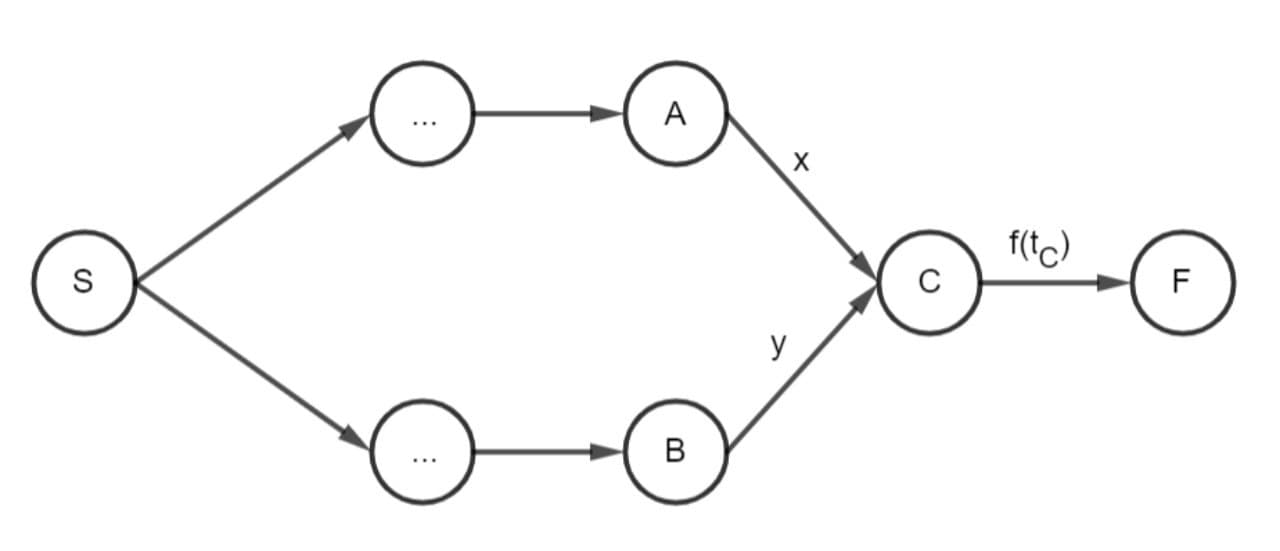
\includegraphics[scale=0.3]{graph_1.jpg}
\end{center}

Без ограничения общности, будем рассматривать часть маршрута P от точки C до F как одно ребро : C-F. Тогда время прохождения этого ребра $\phi(t_C) = \phi_{CF}(t_C)$, где $t_C$ - время старта из точки $C$. Вспомним неравенство прохождения для ребер (см. выше) : $\phi(t_a) \le (t_b - t_a) + \phi(t_b)$, где $\Delta = (t_b - t_a)$

Рассмотрим два маршрута $P : S-...-B-C-F$ и $P': S-...-A-C-F$.
Посчитаем время : $T(P) = t_b + \phi(t_b)$  и $T(P') = t_a + \phi(t_a)$
Используя неравенство, получаем : $T(P') = t_a + \phi(t_a) \le t_a + (t_b - t_a) + \phi(t_b) = T(P)$ Значит маршрут P не является минимальным.

\end{proof}

Понятно, что если неравенство прохождения ребер не выполняется, то модифицированный алгоритм Дейкстры может построить не кратчайший маршрут в терминах временных затрат. Рассмотрим такой пример (рис. 1):
\begin{align*}
	p_1: & \\
	& t_0 = 0 \\
	& \phi_{AC}(t) = 1  \\
	& \phi_{CB}(t) = 1 + 2 * \mathbb{I} \{t < 1.5\} \\
	p_2: & \\
	& t_0 = 0 \\
	& \phi_{AC}(t) = 2  \\
	& \phi_{CB}(t) = 1 + 2 * \mathbb{I} \{t < 1.5\} 
\end{align*}
Время прохождения пути $p_1$ будет составлять $t_{p_1} = t_0 + \phi_{AC}(t_0) + \phi_{CB}(\phi_{AC}(t_0)) = 1 + 3 = 4 $. Время прохождения пути $p_2$ будет составлять $t_{p_2} = 2 + 1 = 3 $. Очевидно, на путь $p_2$ потребуется меньше времени, чем на путь $p_1$, но алгоритм Дейкстры предложит в качестве решения задачи маршрут $p_1$.

\begin{figure}[!hbp]
	\centering
		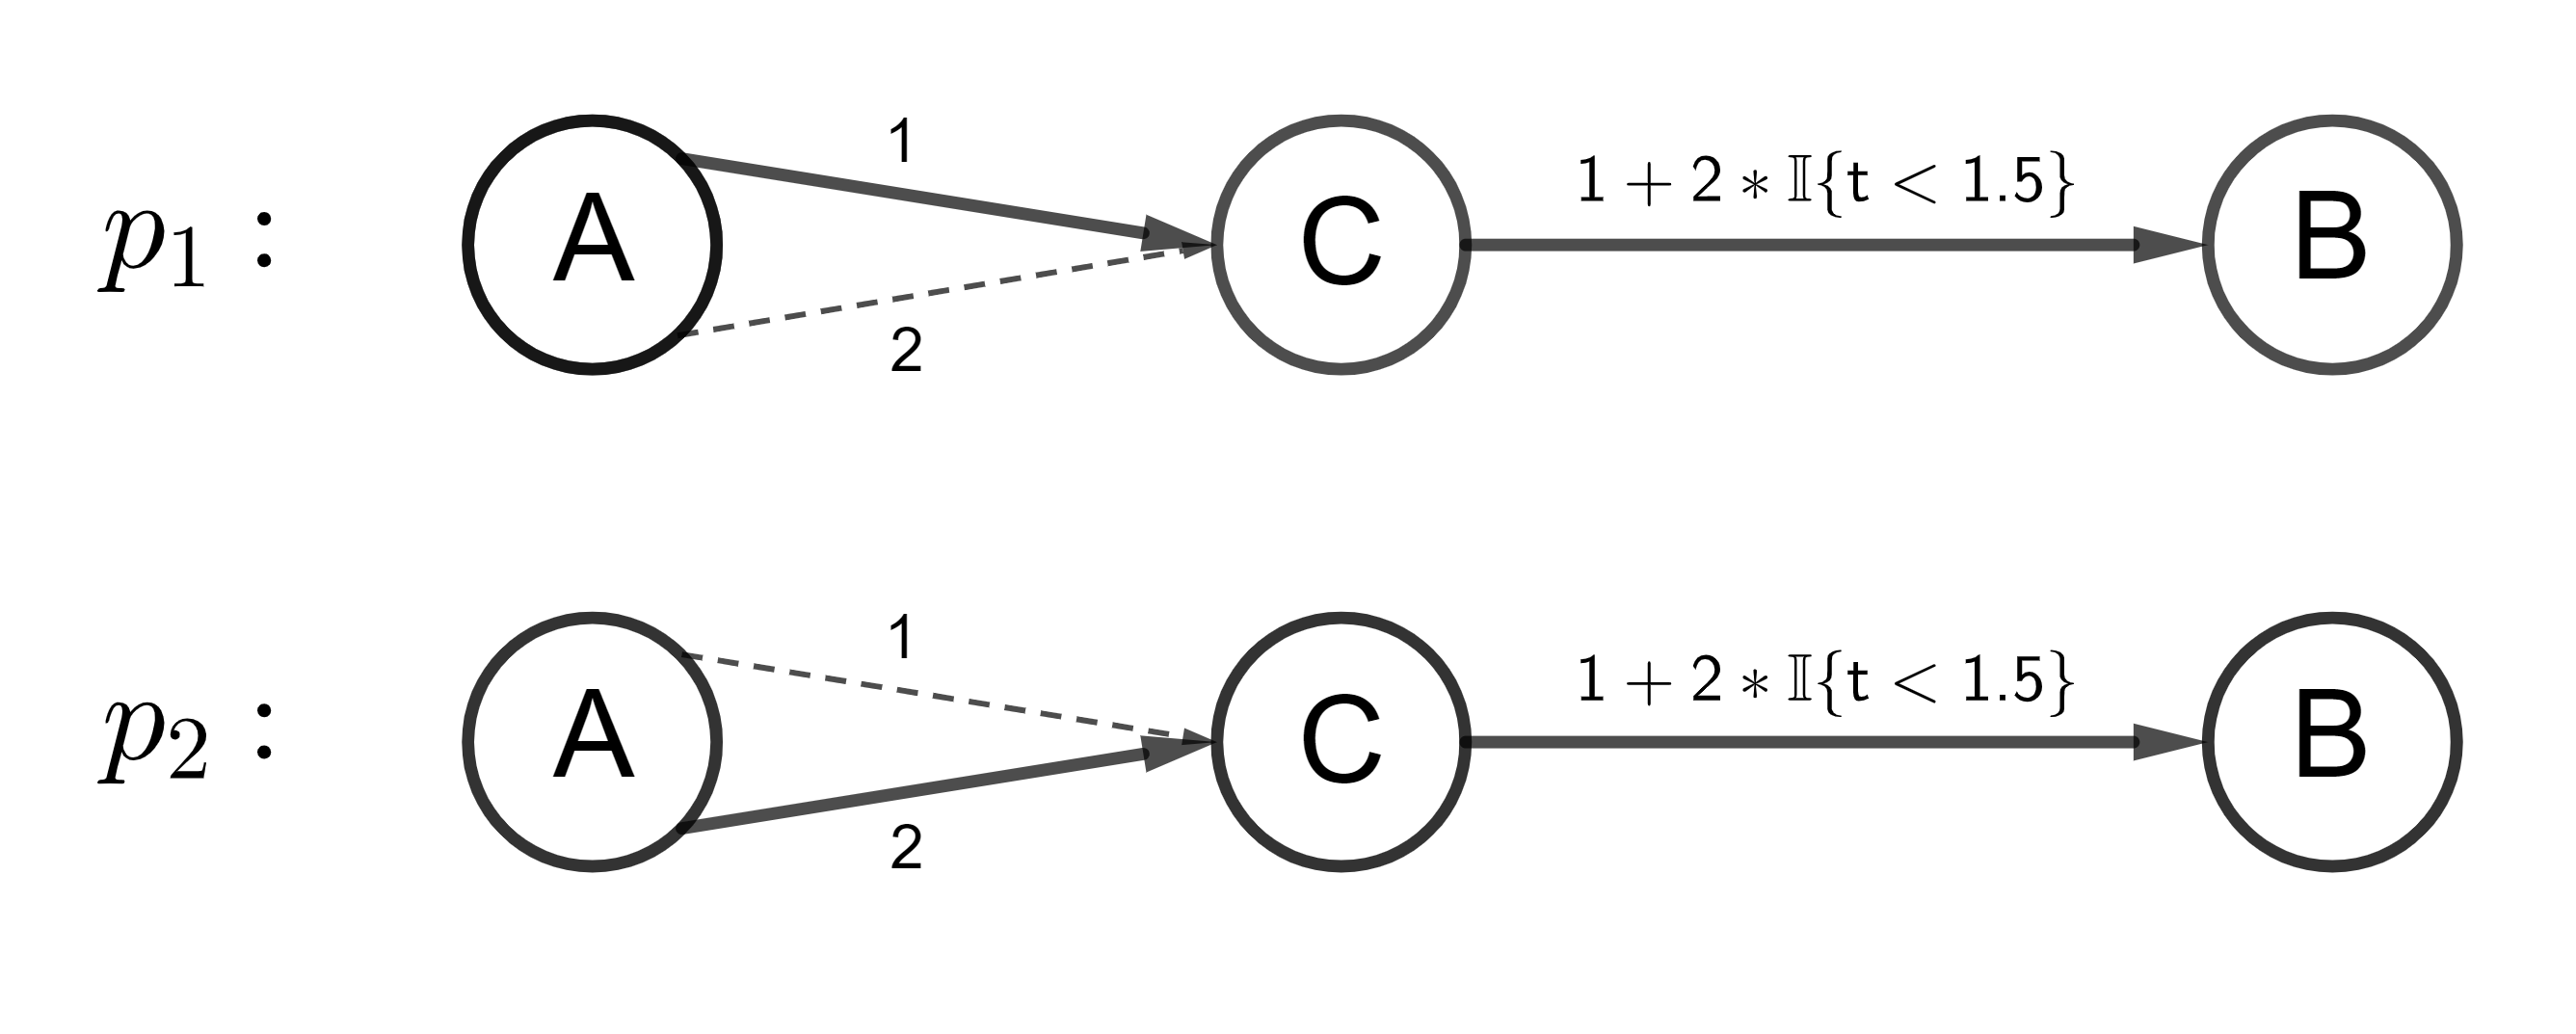
\includegraphics[scale=0.2]{graph_2.png}
	\caption{Пример графа с невыполненным условием неравенства прохождения ребер}
\end{figure}

Отметим, что наша задача поиска оптимального маршрута сводится к вспомогательной задаче. Правила движения участников и их взаимодействий определяют функции $\phi_e$, $e \in E $. Мы можем их получить путем численного моделирования. Неравенство прохождения ребер можно переформулировать так: дорожная сеть обладает условием FIFO --- первый въехавший на дорогу первым ее покидает. Другими словами, если участники не обгоняют друг друга, то путь с минимальными затратами можно найти при помощи алгоритма Дейкстры.


$\textbf{Сложность модифицированного алгоритма Дейкстры}$



\newpage
\section*{Устойчивость нашего решения}



\newpage
\section*{Практические результаты}


\newpage
\section*{Сложность решения}

\newpage
\section*{Альтернативные подходы}

\newpage
\section*{Заключение}

    \newpage
\begin{thebibliography}{0}
	
	\addcontentsline{toc}{section}{Литература}
	
	\bibitem{automat_baza} \textit{Nagel K., Schreckenberg M.} A cellular automation model for freeway
	traffic // Phys. I France. 1992. V. 2. P. 2221–2229.
	
	\bibitem{automat_phyz} \textit{Chowdhury D., Santen L., Schadschneider A.} Statistical physics of vehicular
	traffic and some related systems // Phys. Rep. 2000. V. 329.
	P. 199–329.
	
	\bibitem{automat_jam} \textit{Nagatani T.} The physics of traffic jams // Reports on Progress in Physics.
	2002. V. 65. P. 1331–1386.
	
\end{thebibliography} 

\end{document}